\documentclass[conference]{IEEEtran}
\IEEEoverridecommandlockouts
% The preceding line is only needed to identify funding in the first footnote. If that is unneeded, please comment it out.
\usepackage{cite}
\usepackage{amsmath,amssymb,amsfonts}
\usepackage{algorithmic}
\usepackage{graphicx}
\usepackage{caption}
\usepackage{textcomp}
\usepackage{xcolor}
\usepackage[utf8]{inputenc}
\usepackage{tabularx}
\def\BibTeX{{\rm B\kern-.05em{\sc i\kern-.025em b}\kern-.08em
    T\kern-.1667em\lower.7ex\hbox{E}\kern-.125emX}}
\begin{document}

\title{Development and Application of Drones in Education: A STEAM Approach in Educational Robotics}

%%\author{Gustavo da Silva Nascimento Costa$^{1}$, João Vitor Nascimento$^{2}$, Jeovana Miranda Souza$^{3}$, Rafael Gomes de \\ Oliveira$^{4}$, Sávio Pessôa Afonso$^{5}$, Rian Cesar Oliveira Souza$^{6}$, Leandro Gonçalves dos Santos$^{7}$, \\and Fábio Santos Lima$^{8}$}

\maketitle
\let\thefootnote\relax\footnote{\\979-8-3315-5288-6/25/\$31.00\textcopyright2025 IEEE}

\begin{abstract}
The Educa Drones project, developed by the Baiano Federal Institute - Guanambi Campus, applies the STEAM approach (Science, Technology, Engineering, Arts, and Mathematics) in an interdisciplinary practical learning environment. Focused on the use of rotary-wing drones, such as the Colibri versions, the project allows students and teachers to explore complex concepts by building and operating these aircraft, applying them in pedagogy and student competitions. The initiative enhances learning and encourages innovation.
\end{abstract}

\begin{IEEEkeywords}
Remotely Piloted Aircraft, Educational Robotics, F450, Multirotor, Quadcopter, Modularity.
\end{IEEEkeywords}

\section{Introduction}

Brazilian education, especially in basic education, faces challenges in capturing students' attention and in their learning and cognitive development styles. These issues are confirmed when observing evaluation research.

The results from the Programme for International Student Assessment (PISA), coordinated by the Organisation for Economic Co-operation and Development (OECD), demonstrate the gap in Brazilian education, where more than 50% of 15-year-olds lack basic knowledge in mathematics, science, and languages \cite{b6}. This situation has been worsening since 2009.

In an analysis, Sassaki et al. \cite{a2} concluded that a large portion of the evaluated students did not complete the test, which relates to the difficulty in understanding and solving the questions, indicating that this gap is more related to cognitive skills.

Given this situation, it is necessary to find ways that encourage students’ learning and cognitive development. The application of the STEAM methodology (an acronym for Science, Technology, Engineering, Arts, and Mathematics), which works through solving interdisciplinary problems, stands out, especially through robotics, captivating the student and allowing them to learn through fun and real challenges.

There are various ways to apply educational robotics. One such underexplored pedagogical resource is the use of Remotely Piloted Aircraft (RPA), commonly known as drones, which allow students not only to create and operate ground robots but also to solve problems beyond the two-dimensional (XY) plane, allowing students to give wings to their imagination (XYZ) \cite{a3}.

Moreover, it is possible to explore concepts in physics and mathematics, such as flight dynamics, force, thrust, Newton's laws, distance, height, angles, trigonometry, among others \cite{b11}, contents that are difficult to assimilate within the traditional teaching paradigm.

Through the construction of these devices, it is possible to understand and apply basic and advanced concepts in electronics, chemistry, engineering, and programming \cite{b12}, which are fundamental knowledge for the training of professionals who will be integrated into a globalized market. From this perspective, the Educa Drones project was born at the Federal Institute of Education, Science, and Technology Baiano - Campus Guanambi, located in the productive backcountry, a pioneering initiative in the state. Promoting, through workshops, lectures, student competitions, entrepreneurship, and technological innovation, a stimulating and collaborative environment for teachers and students to train, exchange experiences, and share ideas that result in the development of drones and their insertion into education and other sectors that require their use.

Through this initiative, it was possible to develop the Colibri drones, which play a fundamental role in teaching and in conducting workshops, in addition to contributing to participation in student competitions. These drones enable the dissemination of technological innovations, winning awards, and promoting scientific dissemination, popularization of science, sharing of technical knowledge, strengthening of networks (networking), and cultural exchange.

This article explores the construction and implementation of the Colibri drones in Educa Drones activities, providing a qualitative analysis of their application in the educational context. To address these aspects in more detail, the article is organized as follows: Section 2 presents the Theoretical Framework; Section 3 details the Materials and Methods used; Section 4 presents the Results obtained; and finally, Section 6 discusses the conclusions of the project.

\section{Theoretical Framework}

\subsection{Educational Robotics}

Educational robotics can be defined as a multidisciplinary field of knowledge that applies engineering concepts and other sciences to the design, construction, automation, and control of robotic devices for educational purposes \cite{b1}.

The use of these technological resources for pedagogical purposes in educational institutions has gained increasing interest as educators seek tools to improve teaching and learning processes \cite{b12}. Regarding the application of drones in education, it is essential to recognize that education is a field of constant evolution and innovation. However, there is a noticeable lack of studies and a limited scientific approach to the pedagogical application of drones \cite{b9}.

In support of this perspective, Yepes \cite{b11} notes that while there is abundant material on educational robotics, studies specifically focusing on the use of drones in education are scarce. In the context of educational robotics, drones can be employed as a teaching aid to explore concepts in physics and mathematics, such as flight dynamics, force, thrust, Newton's laws, distance, height, angles, and trigonometry, among others \cite{b11}.

\subsection{Brazilian Legislation on Drones}

According to the Brazilian Civil Aviation Regulation (RBAC-E No. 94), drones with a maximum takeoff weight between 250 g and 25 kg, operating up to 400 feet (approximately 120 meters) above ground level and within visual line of sight (VLOS), are classified as Class 3 \cite{b2}.

Furthermore, as per the National Civil Aviation Agency (ANAC), drones in this class do not need to follow an authorized design or obtain a type certification from the agency. In other words, a certificate of airworthiness is not required. However, operation requires the registration of both the operator and the drone in the Unmanned Aircraft System (SISANT). Compliance with the regulations outlined in RBAC-E No. 94, conformity with the National Telecommunications Agency (ANATEL), and flight authorization from the Department of Airspace Control (DECEA) are mandatory for legal operation \cite{b2}.

\subsection{Student Competitions}

Drone competitions, both in academic and corporate settings, have emerged as favorable environments for the application of educational robotics. Notable examples include the Fórmula Drone SAE Brasil, Drones IFSC, the Brazilian Robotics Competition (CBR), and the most recent initiative, the Bahia Drone Competition.

The Fórmula Drone SAE Brasil is an educational competition focused on the technical development of a radio-controlled rotary-wing aircraft, or drone, equipped with systems designed to complete specific tasks that form the technical challenges of the competition. The primary technological focus is on intelligent onboard systems \cite{b7}. Three editions of the Fórmula Drone SAE Brasil were held (2017, 2018, and 2019) at the UNIFEI Campus in Itajubá, Minas Gerais, but the event was interrupted due to the COVID-19 pandemic. Recently, SAE Brasil announced on its website the return of the competition in 2025 under a new name, EletroQuad, to be held at the University of Vale do Paraíba in São José dos Campos.

The Drone Competition at IFSC Florianópolis Campus has been held annually since 2021 during the National Science and Technology Week (SNCT). This educational competition applies the STEAM concept (Science, Technology, Engineering, Arts, Mathematics) to a technical and technological development activity aimed primarily at high school and undergraduate students. Its goal is to encourage participants to design, assemble, and pilot a battery-powered multirotor drone while completing a series of tasks updated annually in the competition regulations. These tasks challenge participants' problem-solving skills and test the technical capabilities of the drones. Participants' performance is evaluated based on rules outlined in the competition guidelines \cite{b4}.

The Mostra Nacional de Robótica (MNR) [National Robotics Exhibition] is the largest scientific exhibition of robotics projects in Brazil. It targets elementary, high school, technical, undergraduate, graduate students, and researchers, aiming to stimulate, showcase, and promote studies and research in robotics. The best-evaluated projects compete for Junior Scientific Initiation scholarships from CNPQ/MNR, and this project was one of the 60 winners across Brazil in the 2023 edition \cite{b5}.

The Brazilian Robotics Competition (CBR) comprises 16 categories that simulate real-world problems, where autonomous robots (without human intervention) must perform tasks correctly. Among these categories is the RoboCup Flying Robots League, dedicated to autonomous and intelligent drones designed for inspection and operations in pipeline corridors and installations \cite{b3}. This category will feature the participation of the Drones Guanambi team, which will use the Colibri Mini drone currently under development as part of this project. The Colibri Mini will make its public debut at this event.

\subsection{Additive Manufacturing}

Additive manufacturing is a technological tool that can significantly contribute to the application of educational robotics. Its concept emerged in the mid-1980s with the spread of rapid prototyping methodologies, and three-dimensional (3D) printing was one of the possible processes \cite{b10}.

3D printing is essentially the act of transforming raw material from one physical state to another to produce an object, based on a three-dimensional model that is materialized through layer-by-layer deposition \cite{b8}.

It is through this technique that the drones listed below are developed, making it possible to reduce costs and reproduce parts if they need to be replaced.

\section{Materials and Methods}

Remotely piloted aircraft can be either fixed-wing or rotary-wing. In this study, we limit ourselves to the rotary-wing type, which are also called multirotors. For standardization purposes, we refer to these aircraft using the term drone, as they are commonly known.

With this in mind, this section will explore the construction of the structure and the definition of the electronic components of the drones developed in this subproject within the Educa Drones project. These open-hardware initiative models were named Colibri Standard, Colibri Lite, Colibri Mini, Colibri Micro, and Colibri Hexa.


\subsection{Construction Process}

The generic F450 model drone was the starting point for the development of the new aircraft. It features four injection-molded plastic arms, attached with screws to two fiberglass plates to form the frame. In this model, all components are exposed, the wiring is visible, and the aerodynamics are compromised. However, despite its flaws, it is a low-cost option, relatively lightweight, and durable, making it widely used in competitions.

\begin{figure}[!htb]
    \centering
    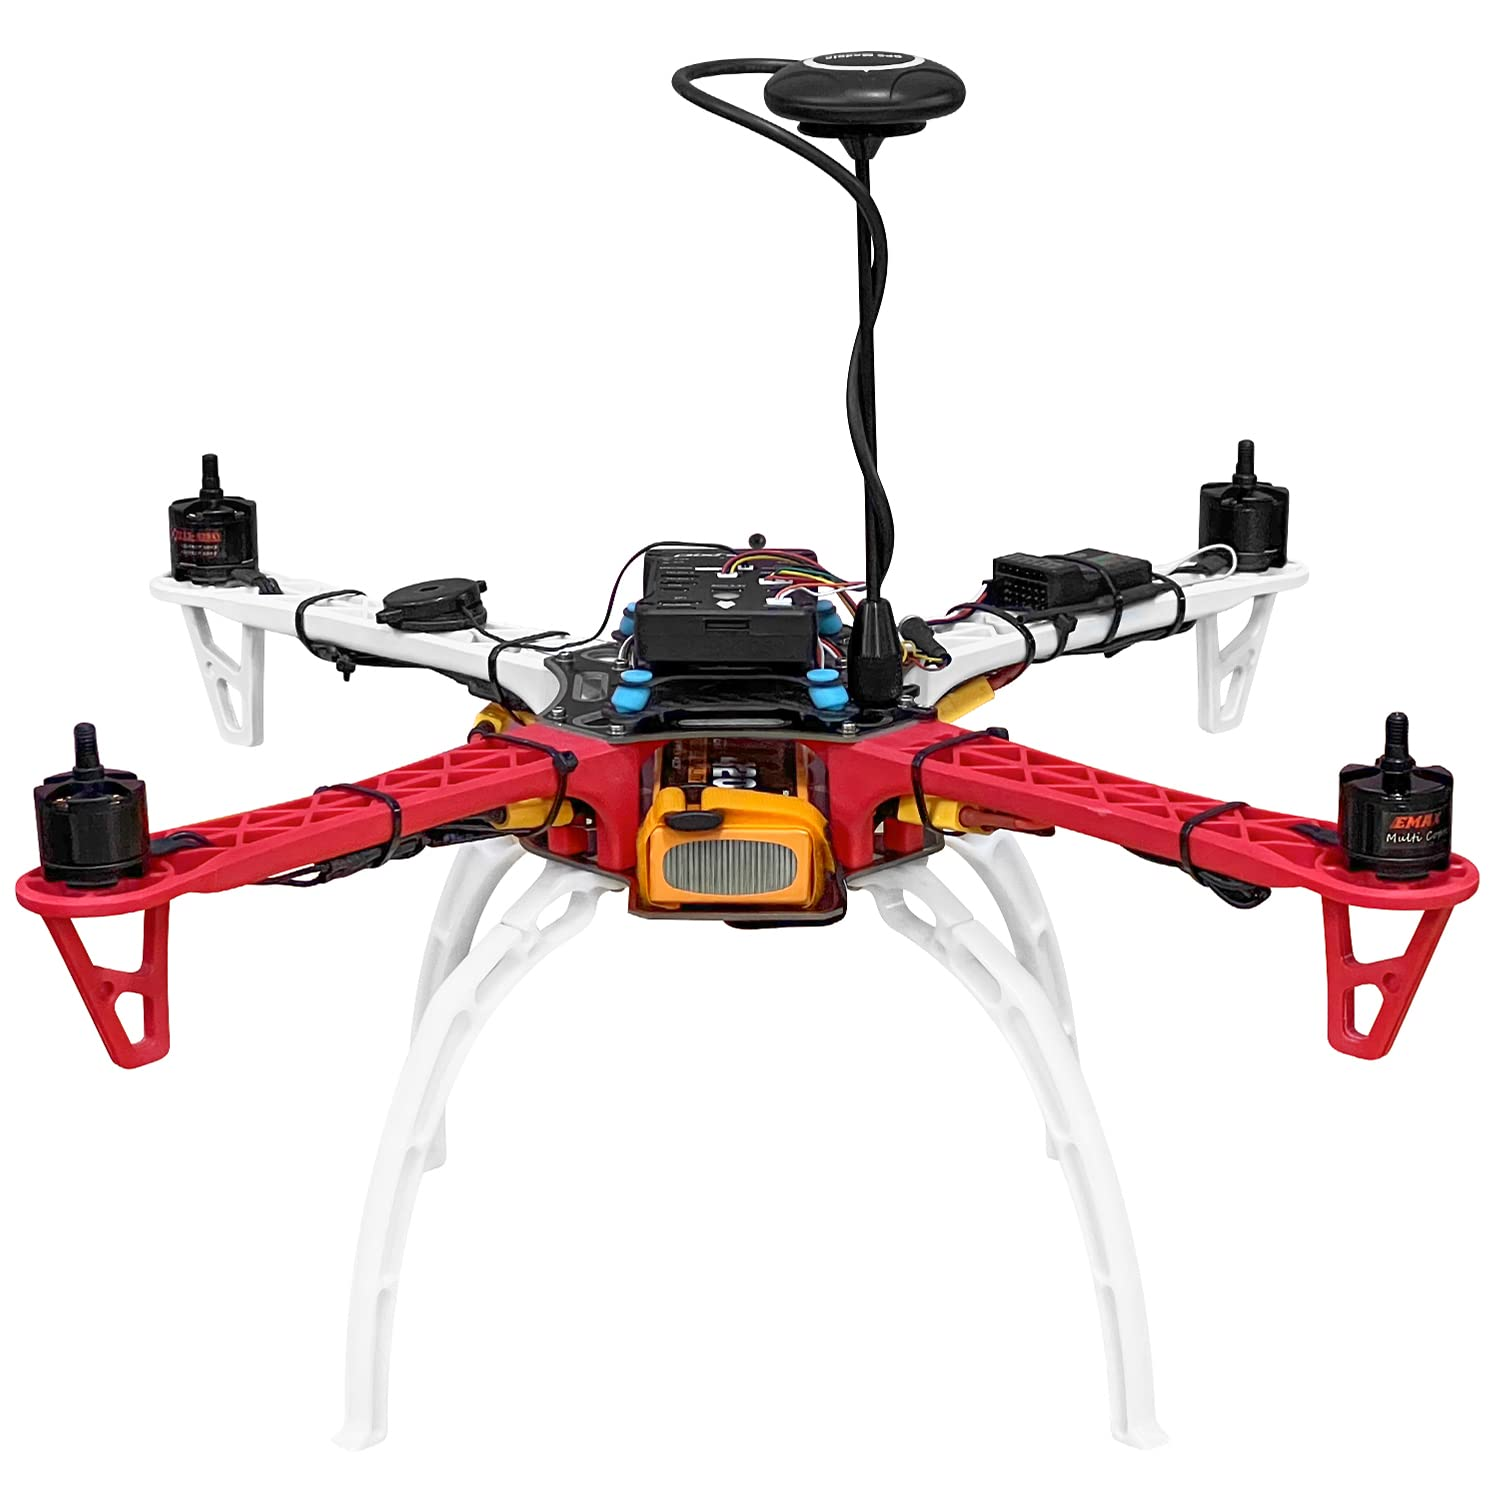
\includegraphics[scale=0.07]{img/f450.jpg} 
    \caption{Generic F450 model. Source: Drones Company.}
    \label{fig:F450}
\end{figure}

After understanding its limitations, the modeling of drones was initiated to correct its flaws while maintaining its positive aspects. Additionally, the modularity criterion was included to facilitate the exchange of components, as well as a safe and appropriate compartment for fitting the batteries. The three-dimensional modeling was developed on the Tinkercad platform, a free online tool that can be accessed through a web browser and does not require a powerful machine to operate.

After the parts were made, the project file was exported in '.STL' format to be sliced into layers in the FlashPrint program. This program is responsible for creating the '.GX' file, which is recognized by the printer to perform layer-by-layer extrusion until the manufactured object is completed.

The new parts were printed using PETG polymer with Guider IIs printers from the manufacturer Flash Forge, and the A2v2 Core printer from the manufacturer GTMax3D. The PETG filament was chosen for its durability, toughness, flexibility, lightweight, and impact resistance in the manufactured objects.

\subsection{Colibri Standard Model}

The drone is named after a hummingbird: Colibri, in homage to the city of Guanambi (hummingbird in Tupi), with the suffix 'standard' because it is the reference model for the other versions. The shape of the central body of the frame was inspired by the generic F450, although with some strategic modifications to better accommodate the electronic components (Figure \ref{fig:F450}).

\begin{figure}[!htb]
    \centering
    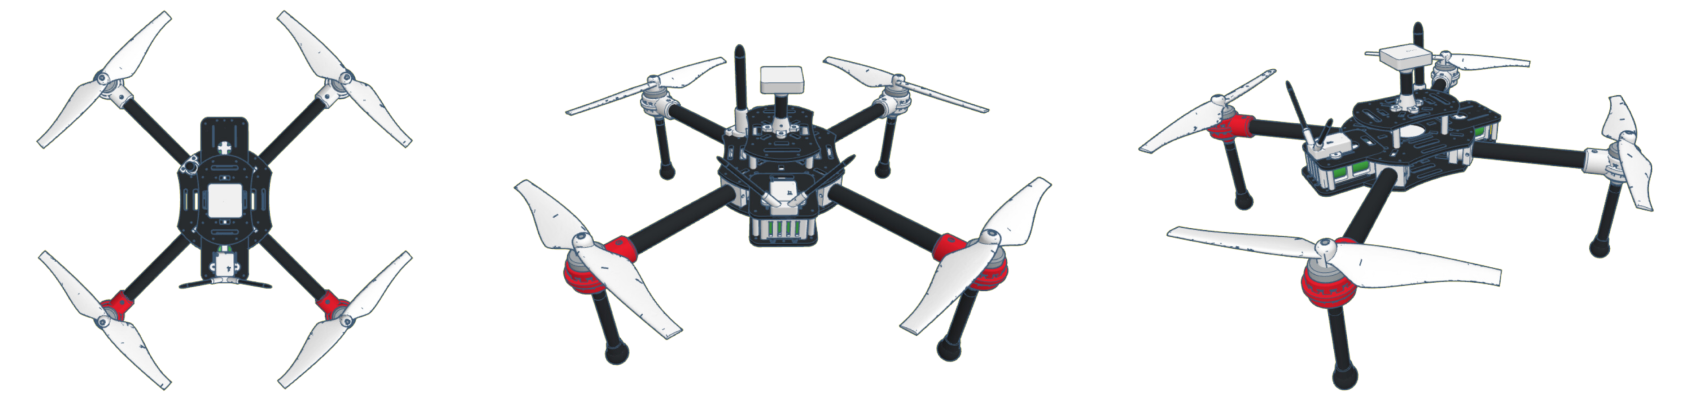
\includegraphics[scale=0.14]{img/Colibri-standard.png} 
    \caption{Three-dimensional model of the Colibri Standard drone in TinkerCad. Source: Author.}
    \label{fig:ColibriStandard}
\end{figure}

It maintains a distance of 450 mm between the axes and a similar-shaped center, using 16 mm carbon fiber tubular arms, which provide strength and protection for wires and devices that can be inserted inside. The landing gear is also made from carbon fiber tubes, with a diameter of 12 mm and a thickness of 1 mm.

Additionally, it features several pre-defined holes that allow for the integration of various accessories such as sensors and robotic mechanisms.

\subsection{Colibri Lite Model}

The Colibri Lite has the same dimensions between the rotor axes as its Standard version, but with modifications to the central body structure prioritizing weight reduction. It was designed for competitions where weight significantly influences the score, but where drones of smaller dimensions are not allowed.

\begin{figure}[!htb]
    \centering
    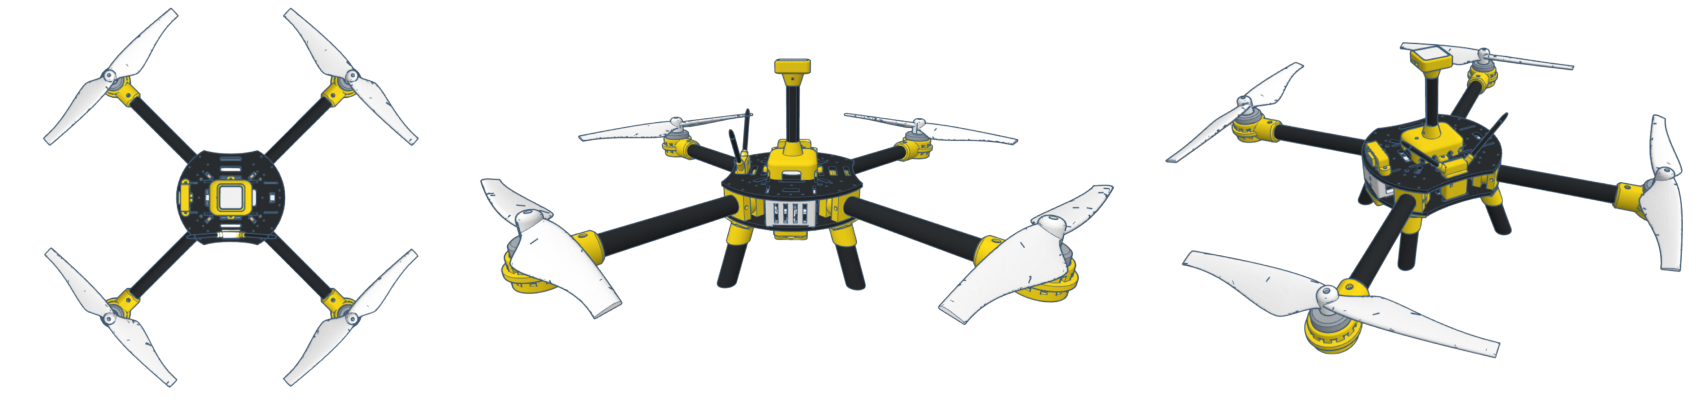
\includegraphics[scale=0.14]{img/Colibri-lite.png} 
    \caption{Three-dimensional model of the Colibri Lite drone in TinkerCad. Source: Author.}
    \label{fig:my_label}
\end{figure}

\subsection{Colibri Mini Model}
The Colibri Mini is a model with 330 mm between the motor axes. It features 12 mm diameter and 1 mm thickness carbon fiber tubular arms, making it generally a scaled-down version of the Colibri Lite.

Its development was initiated with the intention of being used in competitions where drones smaller than 450 mm are the only ones allowed. Although it has a standard size of 330 mm, this dimension can be modified as needed.

\begin{figure}[!htb]
    \centering
    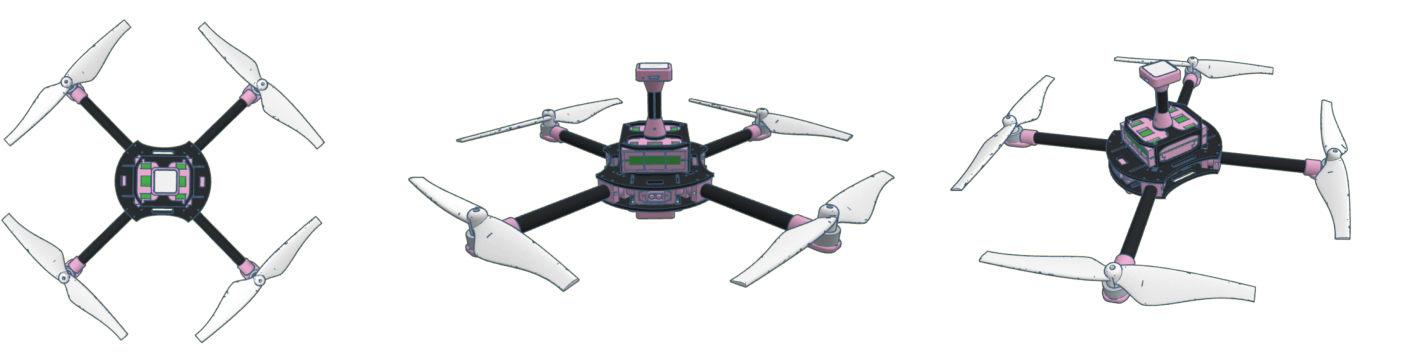
\includegraphics[scale=0.14]{img/Colibri-mini.png} 
    \caption{Three-dimensional model of the Colibri Mini drone in TinkerCad. Source: Author.}
    \label{fig:ColibriMini}
\end{figure}

\subsection{Colibri Micro Model}

The Colibri Micro is the most compact and lightweight model in the Colibri series, with a distance of 188 mm between the motor axes. It is the only one to feature a structure entirely made through additive manufacturing.

Developed for aerial missions in confined spaces or areas with numerous obstacles, its robust and natively integrated propeller protection allows for lower vulnerability to damage and greater safety for animals and people.

\begin{figure}[!htb]
    \centering
    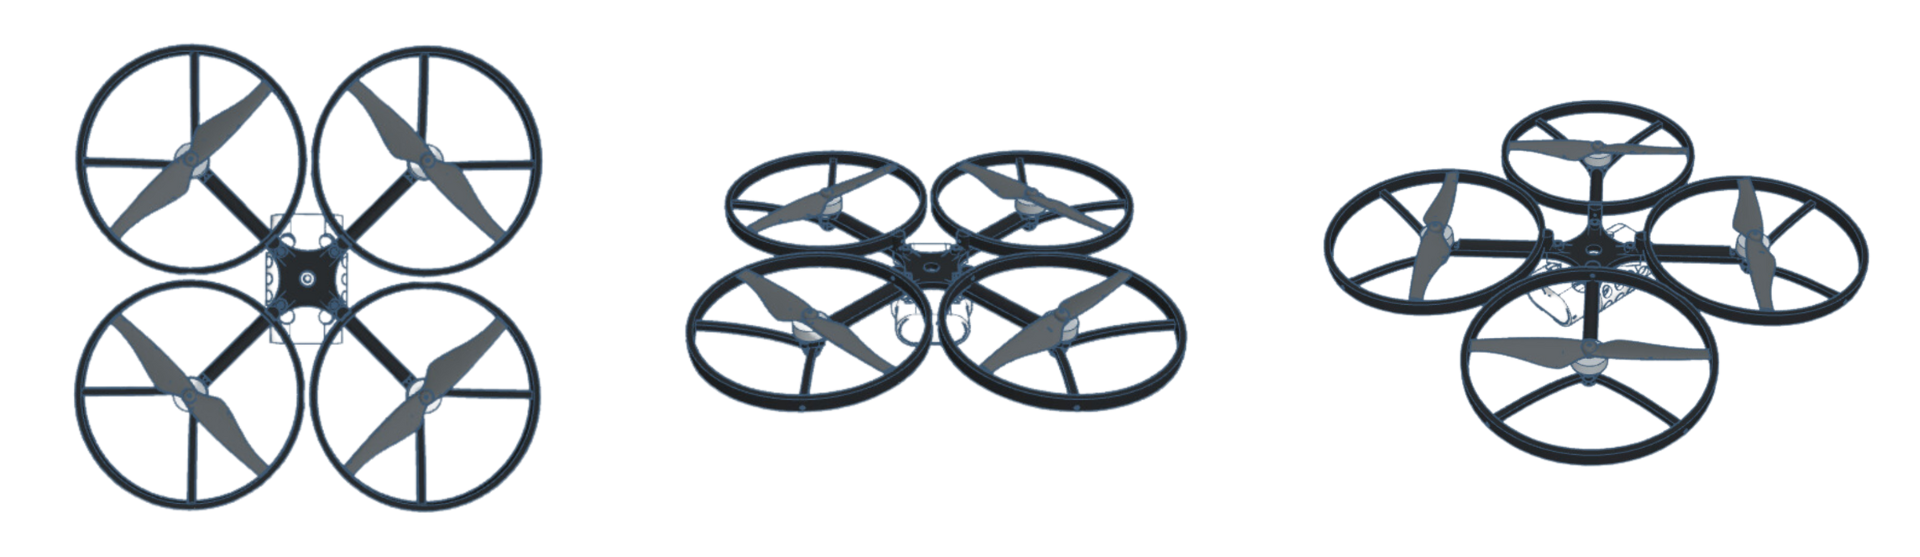
\includegraphics[scale=0.12]{img/Colibri-micro.png} 
    \caption{Three-dimensional model of the Colibri Micro drone in TinkerCad. Source: Author.}
    \label{fig:my_label}
\end{figure}

\subsection{Colibri Hexa Model}
The Colibri-Hexa is the largest in its line, with 6 rotors and 550 mm distance between opposite rotors and 60° between each subsequent arm. As with the other versions, this model features carbon fiber tubular arms with a diameter of 16 mm.

\begin{figure}[!htb]
    \centering
    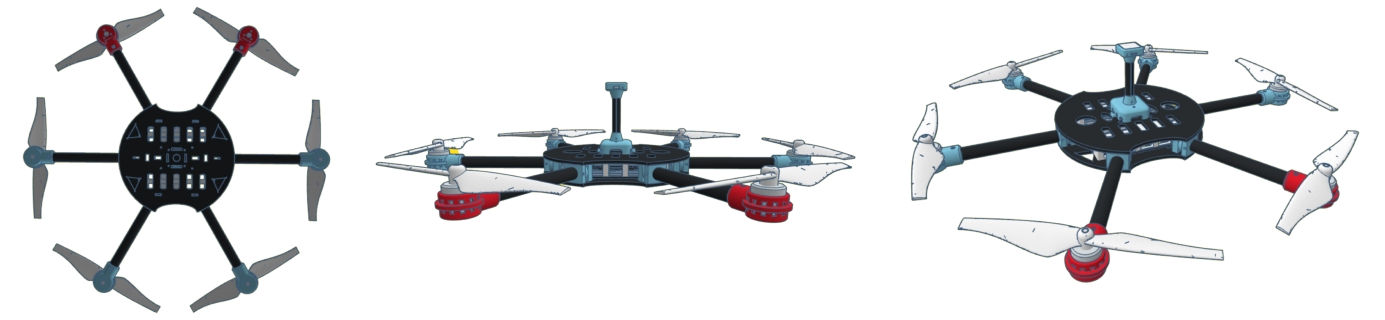
\includegraphics[scale=0.14]{img/Colibri-hexa.png} 
    \caption{Three-dimensional model of the Colibri Hexa drone in TinkerCad. Source: Author.}
    \label{fig:my_label}
\end{figure}

The existence of six motors provides the drone with greater stability and redundancy, allowing the aircraft to remain in flight even if one of them fails. Additionally, it is capable of operating with added weight, which enables the integration of more robust equipment.

\subsection{Electronic Components}

This topic briefly and technically addresses the propulsion system, flight controllers, integrated sensors, and other essential components that contribute to the functionality and performance of these unmanned aerial vehicles.

All versions of the drones developed share similar electronic components, such as the Electronic Speed Control (ESC), which uses BLHeli or SimonK firmware, and is connected to a 32-bit flight controller configured with Ardupilot firmware.

As for the rotors, brushless motors of 800 KV, 1400 KV, and 2824 KV are used, with a relationship inversely proportional to the size of the structure and the propeller.

All batteries are custom-made for each model, using lithium-ion cells with varying capacities and a nominal voltage of 3.7 volts.

For telemetry, all versions use the ESP32 module running Drone Bridge firmware. In combination with a 2.4 GHz WiFi router, this setup allows for bidirectional and encrypted MAVLink communication between the drone and the control station (computer or smartphone).

The GNSS positioning system used in all versions is equipped with the Ublox-M10050 receiver chip and QMC5883L magnetic sensor. This system operates at a higher frequency than normal and supports all GNSS L1 signals (GPS, GLONASS, Galileo, BeiDou), three of which can be used simultaneously and can use up to 32 satellites for navigation with a 10 Hz update rate.

\section{Results and Discussions}

\subsection{Aircraft Performance}

\begin{table}[htbp]
\centering
\caption{Comparison of Drone Models}
\label{tab:drone_comparison}
\begin{tabularx}{\columnwidth}{|l|X|X|X|}
\hline
\textbf{Model}         & \textbf{Operating Weight} & \textbf{Flight Time} & \textbf{Telemetry (Range)} \\ \hline
Colibri Standard       & 1040 g                    & 28 min               & +300 m                     \\ \hline
Colibri Lite           & 788 g                     & 12 min               & +300 m                     \\ \hline
Colibri Mini           & 501 g                     & 28 min               & +300 m                     \\ \hline
Colibri Micro          & 275 g*                    & -                    & +300 m                     \\ \hline
Colibri Hexa           & -                         & -                    & +300 m                     \\ \hline
\end{tabularx}
\newline
\small *Estimated Weight
\end{table}

The Standard model has the highest weight among the 450mm drones tested, at 1040 grams. In contrast, the Lite is the lightest among the 450 class drones, weighing 788 g. Weight reduction is a critical factor, especially in competitions where lightness can significantly improve the score. For competitions where the size of the aircraft is not limited, the Colibri Mini, Micro, and Hexa versions become great alternatives, with the first two designed for indoor competitions with multiple obstacles and the latter where payload and flight stability become crucial for a good score.

Among the 450 class drones, the Colibri Standard achieved the longest flight time, with 28 minutes. In contrast, the Colibri Lite has a significantly shorter flight time of only 12 minutes due to its smaller battery capacity. The Colibri Mini also achieved 28 minutes of flight time despite having a smaller battery. The reason is that its weight is 34.3\% lower than the Colibri Standard.

All models have a telemetry range capacity of +300 m, indicating robust communication sufficient for most field applications. This range is suitable for operations in areas smaller than 9 hectares.

\subsection{Pedagogical Application}

The pedagogical use of the developed drones was implemented through fairs, exhibitions, workshops, and training sessions, often led by the students participating in the project as a form of mutual learning.

Through research and teaching activities, students from the Guanambi campus have the opportunity to work on technological development activities, such as the present study. These initiatives encourage students to engage in the exact and natural sciences in a spontaneous and organic way.

One of the results of this encouragement occurred in 2023, when a high school student from the institute, a participant in the Educa Drones project, was awarded a scientific initiation scholarship from the National Robotics Exhibition. This demonstrates the quality of education when enhanced by pedagogical resources.

\begin{figure}[!htb]
    \centering
    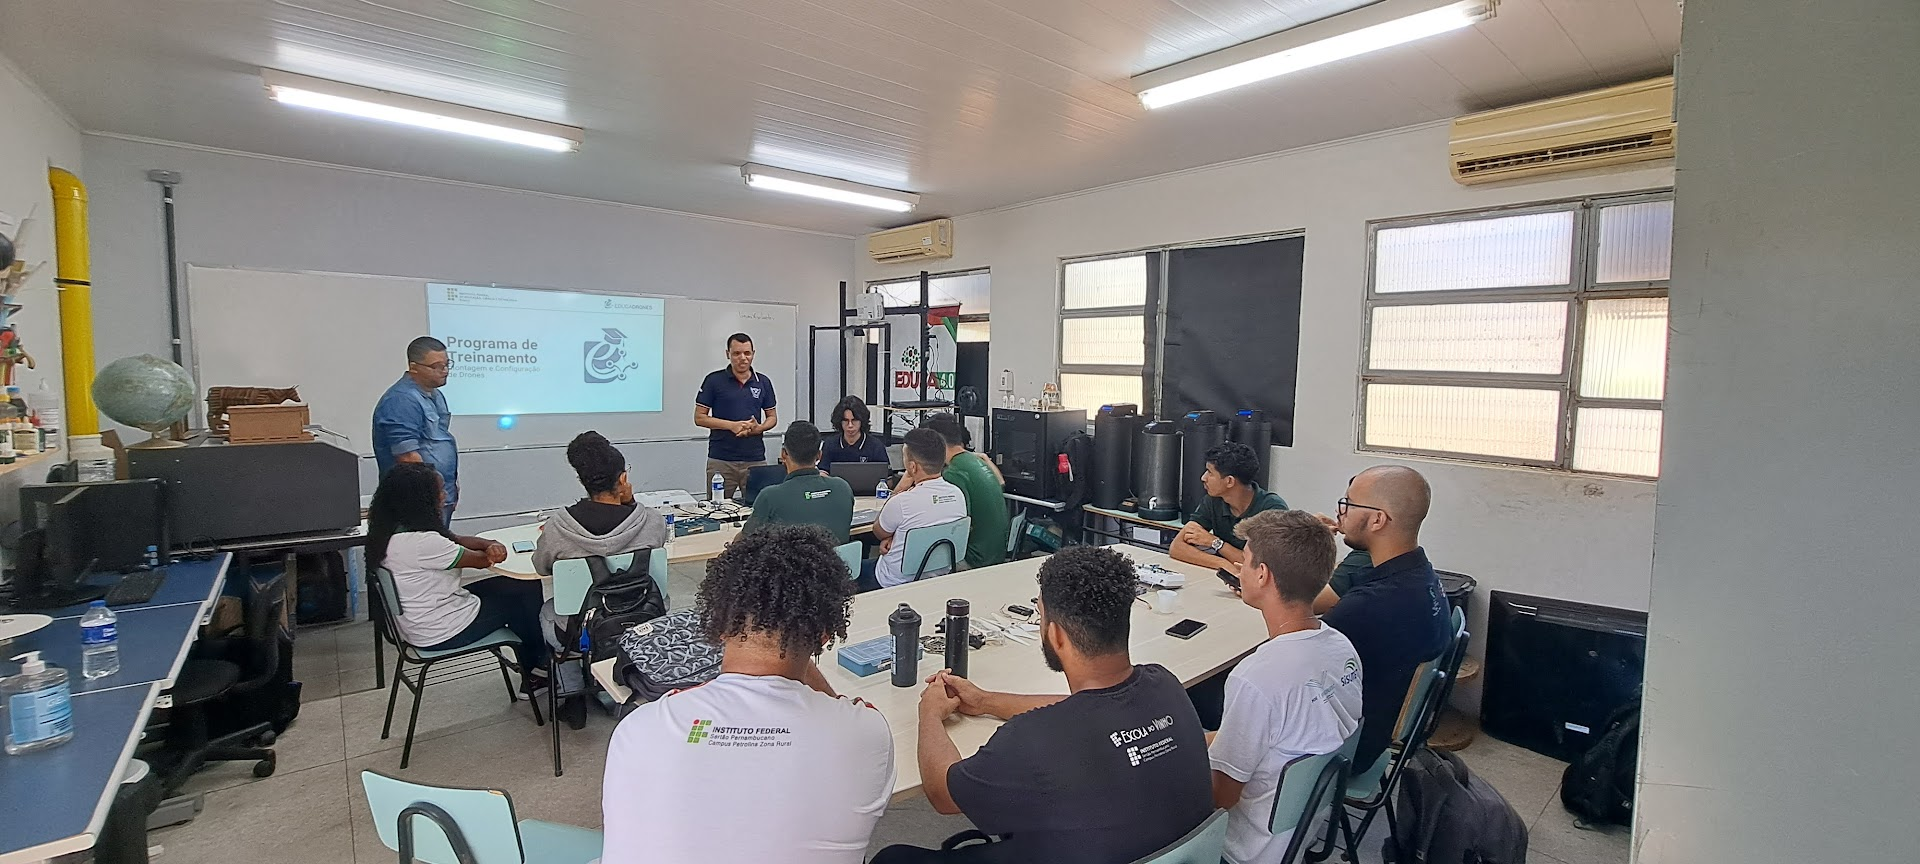
\includegraphics[scale=0.12]{img/petrolina.jpg} 
    \caption{Drone Assembly and Configuration Training in Petrolina-PE. Source: Author.}
    \label{fig:petrolina}
\end{figure}

Also noteworthy is the training program 'Drone Assembly and Configuration,' taught by the professor from IF Baiano Campus Guanambi, Leandro G. dos Santos, and by students experienced in aircraft assembly. The goal is to foster innovation in remotely piloted aircraft systems (RPAS) across various IF Baiano campuses, with implementations already carried out at the Catu-BA, Alagoinhas-BA, and Petrolina Zona Rural campuses (Figure \ref{fig:petrolina}) of the Federal Institute of Pernambuco’s Sertão region. The course is also regularly offered at the home campus, with plans to expand to other units of the Federal Network and other interested institutions.

Aimed at high school and undergraduate students, this course in the training program adopts the STEAM methodology, covering legislation, application, assembly, and configuration of drones, integrating theory and practice in a didactic way.

To maintain the interest of participants in events promoted by the project, participation in competitions, such as the National Drone Models Olympiad (ONdDA), is encouraged. The first edition of this competition will take place in 2025. In addition to being beneficial for students, who have the opportunity to meet and learn from other participants, it encourages innovation and scientific development in the country.

Furthermore, IF Baiano Campus Guanambi is working to organize an internal competition, which will bring together all the institutions that participated in the training program and others that are interested, with the aim of putting into practice knowledge from the STEAM methodology, such as horizontal launch, area and perimeter calculation, computer vision, energy efficiency, aerodynamics, among others.

\subsection{Application in Student Competitions}

Student participation in student competitions, in addition to enabling the dissemination of their innovations and the achievement of awards, also provides scientific dissemination, the popularization of science, sharing of technical knowledge, networking, and cultural exchange. Consequently, this interdisciplinary collaboration positively impacts the teaching-learning process, contributing to the academic and civic formation of the students.

\begin{figure}[!htb]
    \centering
    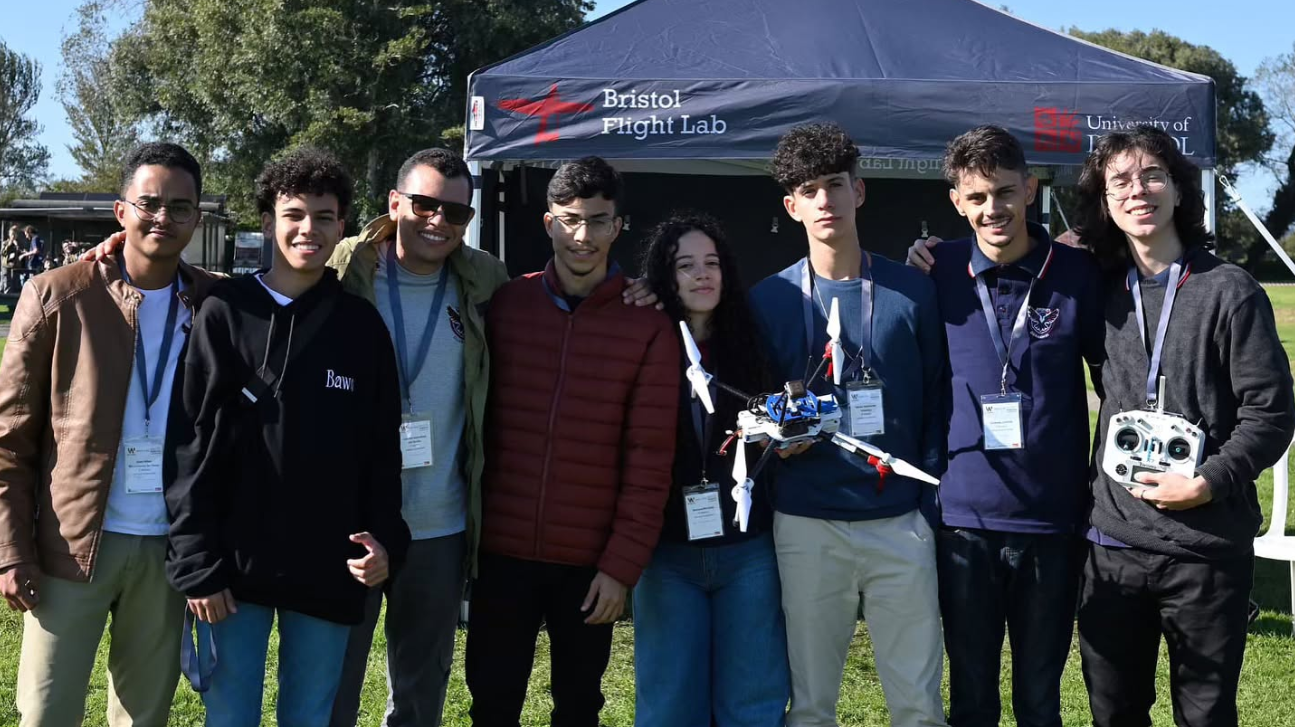
\includegraphics[scale=0.30]{img/imav2024.png} 
    \caption{Drones Guanambi Team in the IMAV outdoor competition. Source: Author.}
    \label{fig:imav}
\end{figure}

As an example, the development of the different drone models presented in this study, integrated with the preparation of the article 'Comparative analysis of cameras for ArUco marker recognition in Unmanned Aerial Vehicles'\cite{a1}, enabled the participation of students from IF Baiano Campus Guanambi in the 2024 International Micro Aerial Vehicles Competition (Figure \ref{fig:imav}), where the Colibri Standard (Figure \ref{fig:ColibriStandard}) was used by the Drones Guanambi team.

\begin{figure}[!htb]
    \centering
    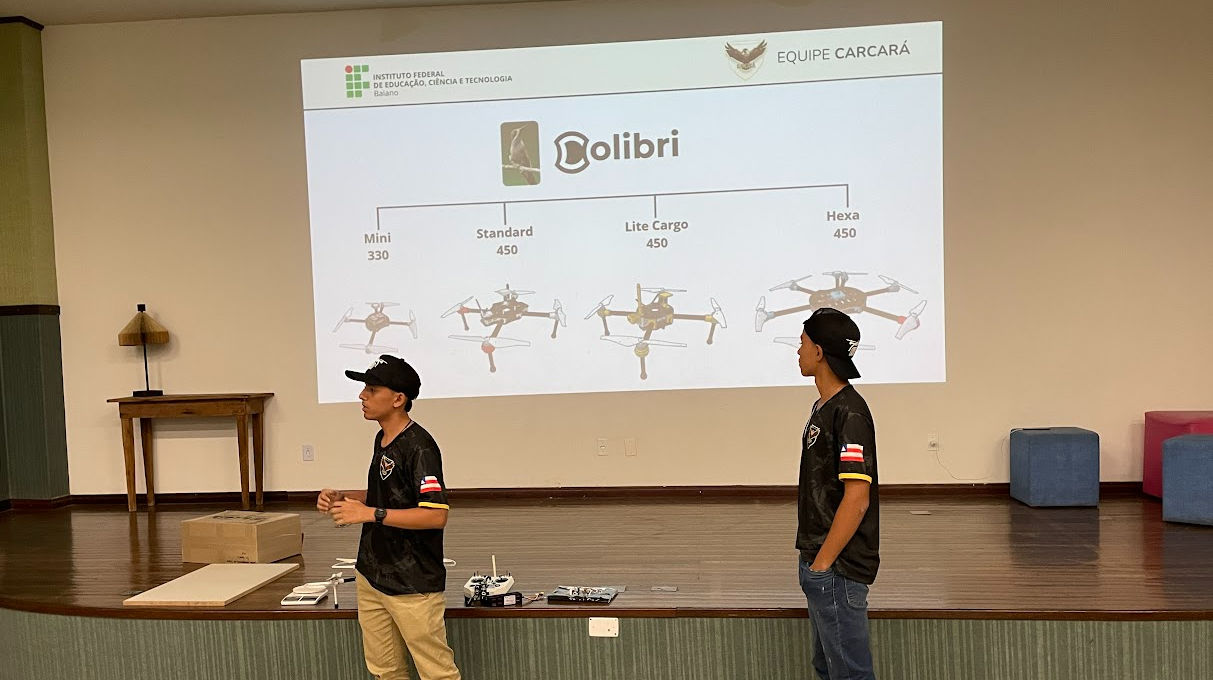
\includegraphics[scale=0.30]{img/ifsc.png} 
    \caption{Technical presentation of the Colibri drones during the Drones IFSC competition. Source: Author.}
    \label{fig:ifsc}
\end{figure}

In the 'Drones IFSC' competition, held in Florianópolis in 2024, students from IF Baiano Campus Guanambi debuted the Colibri Cargo drone, which caught the attention of other competitors and judges (Figure \ref{fig:ifsc}) due to its innovative design and high cargo capacity, finishing the event with a third-place podium position.

Additionally, the challenges proposed in these competitions foster the technological development of the country, encouraging students to create cost-effective solutions to real problems, which, when improved, allow for entry into the commercial sector.

\section*{Final Considerations}

Distinctive characteristics of each drone model developed in the Educa Drones project are highlighted, showcasing their ideal applications based on weight, flight time, and telemetry capabilities. The continuous development and evaluation of these drones can lead to significant improvements in the efficiency and versatility of unmanned aerial vehicles.

For more comprehensive conclusions, additional data from the Colibri Micro and Colibri Hexa models are needed. Future investigations should focus on collecting this data, as well as analyzing resistance, maximum takeoff weight, and stability and flight in adverse wind conditions. Furthermore, a comparison with other commercial drones can provide a broader perspective on the competitiveness of the developed models.

The competitions in which the drones participated revealed both the qualities and flaws of the models used, allowing for the analysis of weak points, including the replacement of the current telemetry with more fault-tolerant systems.

Aimed at the pedagogical applications and student competitions planned for 2025, the use of the drones described here, both in the National Drone Models Olympiad and the internal competition, will enable greater practical observation of the real effects of extension programs and their contribution to the formation of the students involved.

\begin{thebibliography}{00}
    \bibitem{b1} Abreu, J. V. V.; Bastos, B. L. (2015). Robótica Pedagógica e Currículo do Ensino Fundamental: Atuação em uma Escola Municipal do Projeto UCA. Revista Brasileira de Informática na Educação, v.23, n.3, 2015

    \bibitem{b2} Brasil. Agência Nacional de Aviação Civil. (2023). Requisitos gerais para aeronaves não tripuladas de uso civil. RBAC-E94. Emenda n.3. Brasília, 2023.
    
    \bibitem{b3} CBR, Competição Brasileira de Robótica. Disponível em: <https://cbr.robocup.org.br/index.php/categorias/> Acessado em de 30 junho 2024.
    
    \bibitem{b4} IFSC, Competição de Drones IFSC Câmpus Florianópolis. Disponível em: <https://www.ifsc.edu.br/web/campus-florianopolis/veiculos-nao-tripulados-competicao-de-drones> Acessado em de 30 junho 2024.
    
    \bibitem{a1} L. G. dos Santos, J. V. N. Souza, D. F. S. Junio, R. G. de Oliveira, S. P. Afonso, J. M. Souza, F. S. Lima, and R. M. Cotrim, “Comparative analysis of cameras for aruco marker recognition in unmanned aerial vehicles,” in 15$^{th}$ annual international micro air vehicle conference and competition, Bristol, United Kingdom, 2024, p. 177–184.
    
    \bibitem{b5} MNR, Mostra Nacional de Robótica. Disponível em: <https://mnr.robocup.org.br/> Acessado em de 30 junho 2024.
    
    \bibitem{b6} OECD. PISA 2022 Results (Volume I): The State of Learning and Equity in Education. Paris: OCDE Publishing, 2023.
    
    \bibitem{b7} SAE BRASIL. (2020). Fórmula Drone. Disponível em: <http://portal.saebrasil.org.br/programas-estudantis/sae-brasil-helidesign> Acesso: 20 de junho de 2020.
    
    \bibitem{a2} SASSAKI, Alex Hayato; DI PIETRA, Giovanni; MENEZES FILHO, Naercio; KOMATSU, Bruno. Por que o Brasil vai Mal no PISA? Uma Análise dos Determinantes do Desempenho no Exame. Centro de Políticas Públicas do Insper e USP. Policy Paper. n. 31. jun 2018. Insper, 2018. 
    
    \bibitem{b8} Takagaki, L. K. (2012). Tecnologia de impressão 3D. Revista Inovação Tecnológica, São Paulo, v.2, n.2. p.2840. jul./dez.2012. 
    
    \bibitem{b9} Ventura, A. A. O.; Albuquerque, J. L.; Praça Gomes, K. R. F.; Nascimento, S. M.; Leite, E. F.; Alves, J. L.; Diniz, J. R. B.; França, S. V. A. (2022). Robótica educacional e utilização de drones na educação: um mapeamento sistemático da literatura. Research, Society and Development, v. 11, n. 17, e251111739115, 2022.
    
    \bibitem{b10} Wong, K. V.; Hernandez, A. A Review of Additive Manufacturing. ISRN Mechanical Engineering, v. 2012, p. 1–10, 2012
    
    \bibitem{b11} Yepes, I. (2021). Uso de drones como Tecnologia pedagógica em disciplinas steam: um enfoque voltado ao aprendizado significativo com metodologias ativas. Tese (Doutorado) - Universidade Federal do Rio Grande do Sul, Centro de Estudos Interdisciplinares em Pós-Graduação em Informática na Educação. 2021, 240f. 
    
    \bibitem{a3} Yepes, I. (2020). Uso de drones como Tecnologia pedagógica em disciplinas steam: um enfoque voltado ao aprendizado significativo com metodologias
    ativas. Universidade Federal do Rio Grande do Sul-UFRGS.
    
    \bibitem{b12} Yepes, I.; Barone, D. A. C. (2018) Robótica Educativa: Proposta de uso de drones no apoio ao processo pedagógico em disciplinas STEM. Re, v(9). 2018. http://doi.org/10.5281/zenodo.1478926
\end{thebibliography}

\end{document}